\documentclass[11pt]{article}
\usepackage{mathptm,times}
\usepackage[pdftex]{graphicx}
\usepackage[pdftex,
        colorlinks=true,
        urlcolor=linkblue,     % \href{...}{...} external (URL)
        citecolor=linkred,     % citation number colors
        linkcolor=linknavy,    % \ref{...} and \pageref{...}
        pdftitle={LANL Glovebox},
        pdfauthor={Andrew Kurzawski},
        pdfsubject={LANL Glovebox},
        pdfkeywords={UT, LANL, Fire Foe},
        pdfproducer={pdflatex},
        pagebackref,
        pdfpagemode=UseNone,
        bookmarksopen=true,
        plainpages=false]{hyperref}
\usepackage{pdfsync}
\usepackage{color}
\usepackage{titling}
\usepackage[nottoc,notlof,notlot]{tocbibind} % Put the bibliography and index in the ToC

\definecolor{linknavy}{rgb}{0,0,0.50196}
\definecolor{linkred}{rgb}{1,0,0}
\definecolor{linkblue}{rgb}{0,0,1}

\setlength{\droptitle}{-4em}     % Eliminate the default vertical space on the title page.
\addtolength{\droptitle}{5cm}   % Only a guess. Use this for adjustment of the title placement.

\setlength{\textwidth}{6.5in}
\setlength{\textheight}{9.0in}
\setlength{\topmargin}{0.in}
\setlength{\headheight}{0.in}
\setlength{\headsep}{0.in}
\setlength{\parindent}{0.25in}
\setlength{\oddsidemargin}{0.0in}
\setlength{\evensidemargin}{0.0in}

\begin{document}

\pagestyle{plain}

% Project Proposal: Model Calibration and Uncertainty Quantification Using Bayesian Methods

\section{Motivation}
Modeling physical systems requires that we prescribe values for the model parameters based on previous knowledge, correlations, engineering estimations, etc. If we possess expermental data for the system of interest, we can numerically invert for the unknown model parameters. In higher order systems, the solution space may be complicated, and inversion methods can easily get stuck in local minima and maxima. Bayesian inference offers a way to calibrate models of physical systems and calculate the uncertainty in model parameters by using an MCMC sampler.

\section{Experiment and Model}
In previous research, I have examined numerical and experimental use of a coupled-transducer system comprised of thermocouple temperature measurements and time of flight acoustic measurements to determine the recession rate of a carbon material. In the problem of interest, a high heat flux is directed towards the surface of a carbon based material. A temperature profile is set up in the material. Initially the heated face simply increases in temperature with no mass loss. With increasing heating and oxygen transport to the surface, the hot face begins to oxidatively erode. Temperature measurements were made at several locations within the material. During the erosion and heating process a time of flight measurement can also be made in the material with an acoustic transducer. The time of flight depends on temperature and can be modeled by a weighted spatial integration through the material.

Given the temperature measurements and the time of flight measurement, we seek the recession rate. I developed a forward thermal model with a simple representation of oxidation kinetics to describe the process of losing material. Up to this point I have tested several inversion methods on synthetic and experimental data, and while they work reasonably well for predicting the recession rate, there are issues with getting stuck in local minima and not being able to completely recover synthetic data generated by the forward model.

\subsection{Forward Thermal Model}

\begin{figure}[h]
\begin{center}
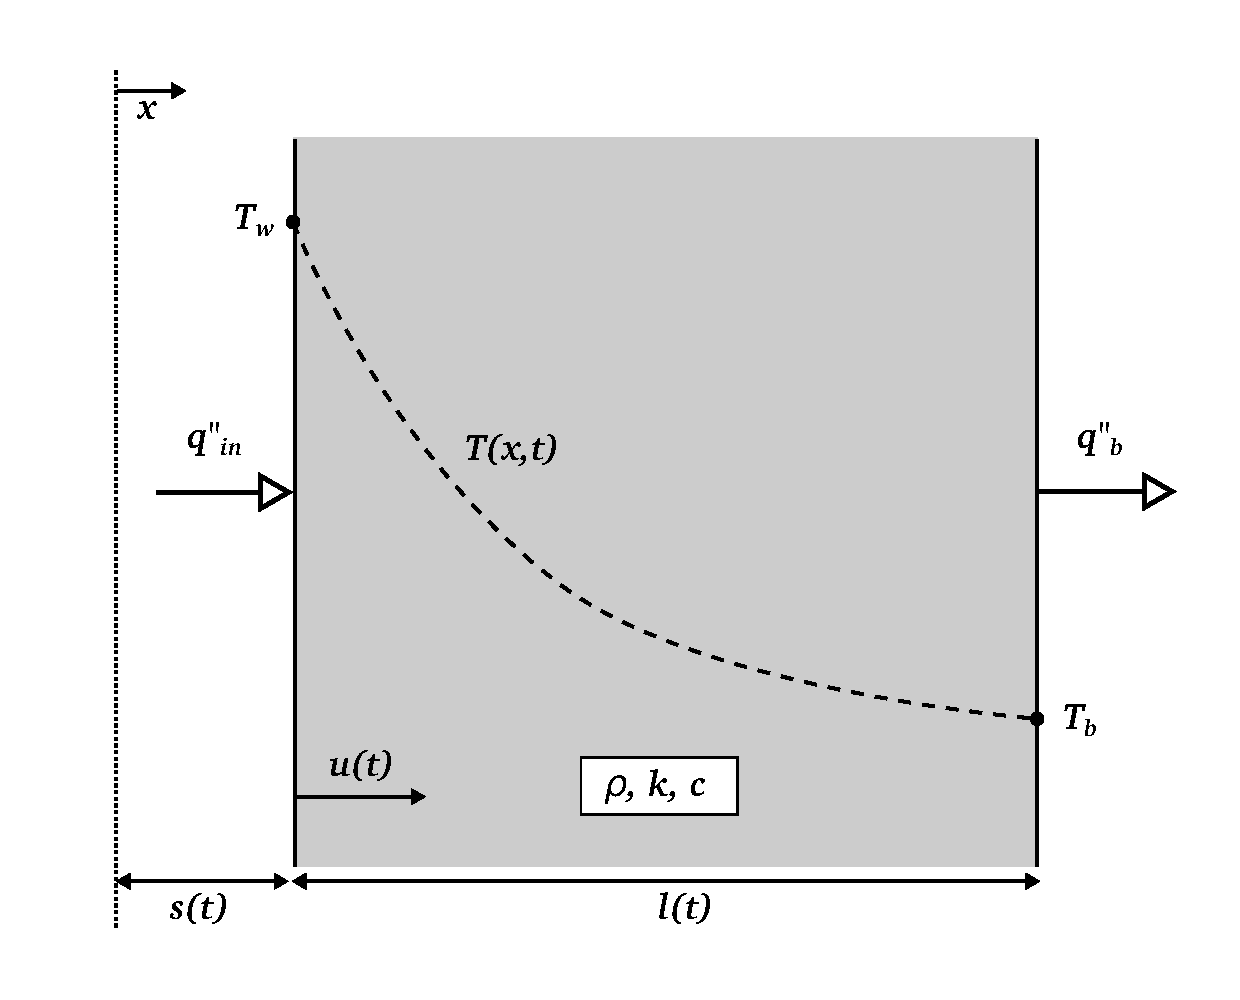
\includegraphics[width=3.4in]{new_abl_sys}
\end{center}
\caption{Schematic of ablating system.}
\label{ablating_system} 
\end{figure}

A simple finite volume model has been constructed for $T(x,t)$ as depicted in Fig.~\ref{ablating_system}, where $T$ is temperature inside the material, $u$ is the recession velocity and $\alpha$ is the thermal diffusivity.

\begin{equation}
\frac{\partial T}{\partial t} - u\frac{\partial T}{\partial x} = \alpha\frac{\partial^2 T}{\partial x^2}
\label{eq_fvmodel}
\end{equation}

Boundary conditions are a prescribed gas temperature, heat transfer coefficient and a mass loss rate specified by an Arrhenius model at $x = 0$. 

\begin{equation}
q''_{in} = -k\frac{\partial T}{\partial x} = h(T_\infty - T_w),\quad x = 0 
\label{eq_bcfront}
\end{equation}

\begin{equation}
m'' = \rho u = A\exp(-T_a/T),\quad x = 0
\label{eq_bcarr}
\end{equation}

The gas temperature and heat transfer coefficient are also prescribed at the back of the model.

\begin{equation}
q''_b = -k\frac{\partial T}{\partial x} = h_b(T_{\infty,b} - T_{w,b}),\quad x = l(t)
\label{eq_bcback}
\end{equation}

Using the forward ablation model, we are able to predict the time of flight and change in time of flight. We can assume that the time of flight measurement takes place over a time period that is small relative to the time for which the spatial temperature variation evolves. As such, the time of flight measurement primarily involves a weighted spatial integration of a function of temperature.

\begin{equation}
\tau(t) = \int_{0}^{l(t)} \frac{dx}{V(T)} = \int_{T(0)}^{T(l)} (\frac{dT}{dx})^{-1} \frac{dT}{V(T)}
\label{eq_tof}
\end{equation}

Our main focus is on predicting the recession rate $u$ in Eqn.~\ref{eq_bcarr}, however we are not able to measure it during the experiment due to the high temperatures. Thus, we are only able to compare the model predicted total recession with the total recession from the experiment.

\section{Project Plan}

My goal is to calibrate the ablation model and quantify uncertainty using data from a set of experiments. Tab.~\ref{tab_para} lists the ``unknown'' parameters in the model. In actuality, I have an idea of the range of these values based on correlations and material handbooks. I plan to experiment with incorporating this knowledge into the priors for these parameters and with using subsets of the full experimental data set. I will be using a package called PyMC, and I would also like to experiment with the different stepping methods included in the package.

\begin{table}[h]
\caption{PARAMETERS}
\begin{center}
  \begin{tabular}{cccc}
    \hline\noalign{\smallskip}
    Parameter & Symbol & Units \\
    \noalign{\smallskip}\hline\noalign{\smallskip}
    Front (Flame) Side Temperature & $T_\infty$ & $K$\\
    Flame Side Heat Transfer Coefficient & $h$ & $\frac{W}{m^2K}$\\ 
    Material Specific Heat & $c$ & $\frac{J}{kgK}$\\ 
    Material Conductivity & $k$ & $\frac{W}{mK}$\\ 
    Back Side Gas Temperature & $T_{\infty,b}$ & $K$\\ 
    Back Side Heat Transfer Coefficient & $h_b$ & $\frac{W}{m^2K}$\\ 
    \noalign{\smallskip}\hline
  \end{tabular}
\end{center}
\label{tab_para}
\end{table}

\bibliographystyle{unsrt}
\bibliography{../../Bibliography/UTFRG_general}

\end{document}
